\documentclass[10pt,letterpaper]{article}
\usepackage[margin=0.8in,headheight=14pt]{geometry}
\usepackage[T1]{fontenc}\usepackage{lmodern,microtype}
\usepackage{amsmath,amssymb,booktabs,array,graphicx,xcolor}
\usepackage{caption,float,enumitem,fancyhdr,xurl}
\usepackage[colorlinks=true,linkcolor=navy,urlcolor=navy,citecolor=navy]{hyperref}
\definecolor{navy}{HTML}{245B89}
\setlength{\parskip}{4pt}\setlength{\parindent}{0pt}
\captionsetup{font=small,labelfont=bf}
\setlist[itemize]{itemsep=2pt,topsep=3pt,leftmargin=17pt}
\pagestyle{fancy}\fancyhf{}
\fancyhead[L]{\small Qwen2.5-3B Reasoning SFT}\fancyhead[R]{\small Project 1 -- Interim Submission}
\fancyfoot[C]{\small\thepage}
\hypersetup{pdftitle={Data Selection and Reasoning SFT: Completed Four-Model Comparison},pdfauthor={Rohit Kumar Salla, Manoj Saravanan, Haissam Adam}}
\title{\vspace{-1.5em}\textbf{Data Selection and Reasoning SFT}\\\large Completed Four-Model Comparison and Project Evidence}
\author{Rohit Kumar Salla \quad Manoj Saravanan \quad Haissam Adam}
\date{October 26, 2026}
\begin{document}\maketitle\thispagestyle{fancy}
\begin{abstract}
We evaluate data-selection strategies for full-parameter supervised fine-tuning of Qwen2.5-3B-Instruct on original AceReason targets. A completed one-epoch comparison uses random and route-selected 15,000-example subsets under the same training settings. Their seven-benchmark mean pass@8 scores are 50.6262\% and 51.5222\%, compared with 49.5474\% for the original model. A separate assistance-and-coverage model reaches 52.4773\% and meets three of nine fixed historical reference targets: AIME 2025, Minerva Math and GPQA-Diamond. All four models complete all nine benchmarks with matching inference settings and hardware. The best model also changes context, learning rate and training duration, preventing selection-only attribution. Its average pass@1 remains below the original and truncation increases substantially. We distinguish measured outcomes, public artifacts and remaining release gaps; no nine-target success, official leaderboard rank or bonus is claimed.
\end{abstract}

\section{Objective and Submission Scope}
The project studies whether selecting diverse, complete-looking original reasoning demonstrations improves multi-sample problem solving over random sampling. Training uses LLaMA-Factory~\cite{llamafactory}, Qwen2.5-3B-Instruct~\cite{qwen} and the assignment's AceReason source~\cite{acereason,assignment}. Lower training loss is treated as optimization evidence, not proof of reasoning quality.

This snapshot contains four completed nine-benchmark evaluations. The core data-selection comparison holds the random and advanced route models' training recipe fixed. The best assistance model is presented separately because its larger context and training budget change the experiment. Ongoing exploratory runs do not contribute scores to this report.

\begin{table}[H]\centering\small
\caption{Submission navigation aligned with the instructor's rubric. Points are available weights, not self-awarded scores.}
\begin{tabular}{p{.42\linewidth}rp{.39\linewidth}}\toprule
Category & Points & Repository evidence\\\midrule
Environment and reproducibility & 10 & README, REPRODUCE, dependencies\\
Dataset preparation & 15 & Preparation, selectors, public datasets\\
SFT implementation and training & 20 & Configs, trainer, finite histories\\
Model evaluation & 20 & Four suites, protocol, CPU verifier\\
Advanced selection & 20 & Method, implementation, random comparison\\
Report and analysis & 15 & This report, tables and figures\\\bottomrule
\end{tabular}
\end{table}
The public repository's \texttt{RUBRIC.md} maps every subcriterion. The existing public model is the 51.5222\% advanced route model. The best model's weights and distinct assistance-selected dataset remain unpublished; their measured results are included without relabeling the existing release.

\newpage
\section{Dataset Preparation and Selection}
\subsection{Shared Preparation and Random Control}
The supplied AceReason-1.1 100K data are normalized to instruction, input, output and optional system fields. Preparation removes invalid examples and normalized duplicate prompts, excludes recognizable benchmark overlaps using exact matches and character shingles, and reserves validation before selection. These operations reduce detectable overlap; they do not prove absence of semantic contamination or pretraining exposure.

The random dataset contains 15,000 source examples sampled with seed 42. The published advanced route dataset also contains 15,000 original examples. Both exports are public in the same Hugging Face dataset repository. Original responses remain training targets; no benchmark answers or generated replacements are used as training labels.

\subsection{Advanced Route Selection: Hypothesis and Implementation}
Our hypothesis is that quality filtering and topic/route coverage reduce redundant demonstrations while retaining useful variation. Eligibility requires at least 128 response tokens, a complete boxed answer, repeated word-eight-gram fraction at most 0.35, and a complete sequence fitting the 8,192-token selection cutoff with a 32-token reserve. For word eight-grams $G_8(y)$, repetition is $1-|\mathrm{unique}(G_8(y))|/|G_8(y)|$, defined as zero if none exist. These are text proxies, not correctness certification.

Prompt features use character TF--IDF, truncated SVD and MiniBatch K-means. The export has 113 populated eligible clusters. Each next quota slot goes to the non-full cluster maximizing $\sqrt{N_j}/(q_j+1)$, where $N_j$ is capacity and $q_j$ the current quota. This balances corpus prevalence against broad coverage.

Within a cluster, 180-dimensional lexical route features encode cue counts, late-response cues, cue transitions and cue presence across 12 families. Standardized, clipped and normalized vectors support greedy farthest-point selection, weighted 80\% toward diversity and 20\% toward low repetition. These features describe solution text, not validated proof graphs. Seed 42 fixes the output shuffle. Eligibility differs between random and advanced, so the comparison tests the whole selection procedure.

\subsection{Best Extension: Assistance-Associated Utility and Coverage}
A distinct dataset uses saved source-only normal-versus-prefix-assisted observations, two supported, normally finished samples per condition. Laplace-smoothed probabilities and utility are
\[
 p_n=(c_n+1)/4,\quad p_a=(c_a+1)/4,\quad
 u=(1-p_n)\max(p_a-p_n,0).
\]
Missing, censored and unsupported measurements remain unscored. Each topic cluster is divided into response-length quartiles; capped square-root quotas permit positive-utility selection for at most half of each cell. Deterministic source-ID ordering fills the rest. The saved selection has 56,673 eligible originals, 23,014 scored prompts, 3,672 utility selections and 11,328 coverage selections. Native preprocessing records 105,389,717 supervised response tokens per epoch.

Training still uses complete original targets. Assistance association is not a causal learnability estimate; semantic prefix leakage has not been excluded. The public portable selector exposes scoring and quota selection, but the exact saved measurement ledger and this separate data export are absent from the current public release. It cannot be reproduced exactly by substituting the published route dataset.

\newpage
\section{SFT Setup and Evaluation Protocol}
\subsection{Completed Training Configurations}
All trained models update full parameters with response-only autoregressive cross-entropy, Qwen template, SDPA attention, BF16 mixed precision and gradient checkpointing. Packing and prompt loss are disabled. Weight decay is 0.01, gradient clipping 1.0 and train/data seeds are 42.

\begin{table}[H]\centering\small
\caption{Core comparison and separate best extension.}
\begin{tabular}{lrrr}\toprule
Setting & Random & Advanced route & Best assistance\\\midrule
Original examples & 15,000 & 15,000 & 15,000\\
Training context & 4,096 & 4,096 & 16,384\\
Epochs & 1 & 1 & 3\\
Optimizer updates & 1,875 & 1,875 & 5,625\\
Effective batch size & 8 & 8 & 8\\
Learning rate & $2\!\times\!10^{-6}$ & $2\!\times\!10^{-6}$ & $5\!\times\!10^{-6}$\\
Schedule & Cosine & Cosine & Cosine\\
Warmup ratio & 0.03 & 0.03 & 0\\\bottomrule
\end{tabular}
\end{table}
The random and advanced recipes use one rank with batch one and accumulation eight. The best recipe uses four ranks with batch one and accumulation two per rank. It completed through recovery across allocations. Saved histories contain every finite update through 1,875 or 5,625 respectively. The histories establish completed optimization; they are not accuracy estimates.

The published random/advanced selection cutoff is 8,192, but their training context is 4,096; some selected targets can be truncated. The original loader did not explicitly map the system column. These are disclosed properties of the completed comparison, not demonstrated causes of its outcomes.



\subsection{Matched Inference and Metrics}
Each of four models completes 1,974 records across AMC, AIME 2025, AIME 2024, MATH-500, CN Math 2024, Kaoyan, Minerva Math, OlympiadBench and GPQA-Diamond. AIME 2025 is a separately sourced supplement. The evaluated MATH denominator is 500. There are eight responses per record, or 15,792 samples per model.

All four suites use one B200, vLLM 0.19.0, Transformers 4.57.6, PyTorch 2.10.0, seed 0 with stable question seeds, temperature 0.6, top-$p$ 0.95, maximum new and total-context limits of 32,768, batch 1,024, maximum active sequences 128, tensor parallelism one and memory utilization 0.85. The original boxed-answer system prompt, extraction and grader are retained. Prompt tokens consume total context.

For $c_i$ correct answers among eight, pass@1 is $\frac{1}{N}\sum_i c_i/8$ and pass@8 is $\frac{1}{N}\sum_i\mathbf{1}[c_i>0]$. The assignment mean equally weights seven tasks, excluding AIME 2024 and MATH. It is neither a pooled-question score nor the mean of all nine.

\newpage
\section{Complete Benchmark Results}
\begin{table}[H]\centering\scriptsize
\caption{Pass@8 in percent for every completed model. The final columns compare the best model's solved count to the fixed integer requirement. These historical targets are distinct from our matched original-model scores.}
\begin{tabular}{lrrrrrrr}\toprule
Benchmark & $N$ & Original & Random & Advanced & Best & Solved/required & Met\\\midrule
AMC & 40 & 77.50 & 77.50 & 70.00 & 70.00 & 28/33 & No \\
AIME 2025 & 30 & 13.33 & 13.33 & 20.00 & 26.67 & 8/8 & Yes \\
AIME 2024 & 30 & 23.33 & 20.00 & 16.67 & 20.00 & 6/8 & No \\
MATH-500 & 500 & 85.20 & 84.20 & 85.00 & 88.20 & 441/451 & No \\
CN Math 2024 & 30 & 23.33 & 30.00 & 33.33 & 33.33 & 10/14 & No \\
Kaoyan & 199 & 56.78 & 55.78 & 59.80 & 66.83 & 133/138 & No \\
Minerva Math & 272 & 49.63 & 46.32 & 48.90 & 47.06 & 128/95 & Yes \\
OlympiadBench & 675 & 49.48 & 49.63 & 49.33 & 52.74 & 356/385 & No \\
GPQA-Diamond & 198 & 76.77 & 81.82 & 79.29 & 70.71 & 140/121 & Yes \\
\midrule
Seven-task mean & -- & 49.5474 & 50.6262 & 51.5222 & 52.4773 & -- & --\\\bottomrule
\end{tabular}
\end{table}

\begin{figure}[H]\centering
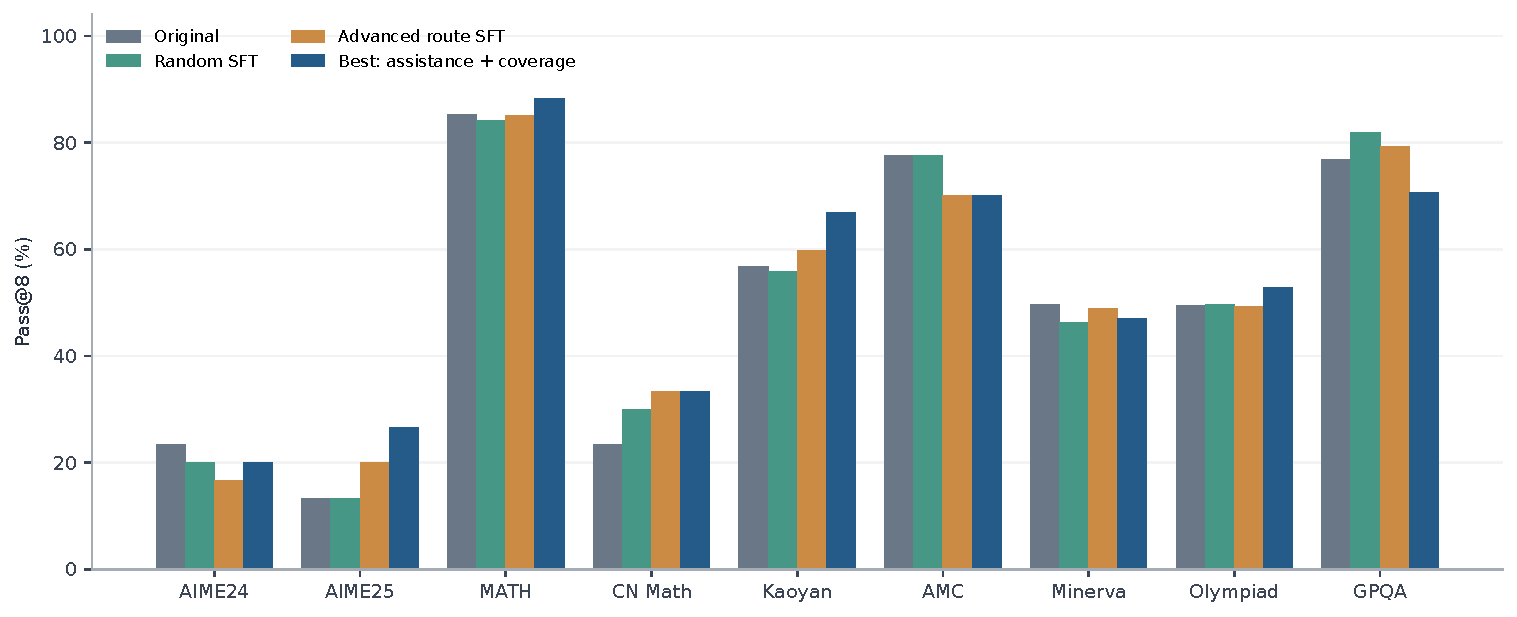
\includegraphics[width=\linewidth]{figures/rubric_benchmarks.pdf}
\caption{All nine pass@8 scores. One fixed best model supplies all its scores; we do not stitch benchmark-specific winners. Complete regressions remain visible.}
\end{figure}

\textbf{Three of nine targets.} The assistance model meets AIME 2025 (8/30), Minerva (128/272) and GPQA (140/198), while missing the other six. The integer targets require strict exceedance of the fixed historical reference percentages. This is a local reference check, not proof of official leaderboard placement. It does not establish eligibility for the top-five bonus.

\textbf{Core selection comparison.} Advanced route SFT exceeds random by 0.8960 percentage points in seven-task pass@8 under the same one-epoch training settings. This is a descriptive single-seed comparison. Different selected examples and response-token exposure remain part of the treatment.

\textbf{Best extension.} The assistance model exceeds random by 1.8510 points and the original by 2.9298 points in the same mean. Context, learning rate, warmup and training duration also change; the difference cannot be attributed solely to assistance-based selection.

\textbf{Regressions.} Relative to our original, the best model decreases on AMC, AIME 2024, Minerva and GPQA. Meeting the Minerva and GPQA historical targets does not imply beating this matched original on those tasks. Nine-target success has not been achieved.

\newpage
\section{Analysis, Limitations and Improvements}
\begin{table}[H]\centering\small
\caption{Metric and generation tradeoffs on the identical completed suites.}
\begin{tabular}{lrrr}\toprule
Model & Mean pass@1 (\%) & Mean pass@8 (\%) & Truncated / 15,792\\\midrule
Original & 23.5497 & 49.5474 & 141\\
Random SFT & 21.1928 & 50.6262 & 2,494\\
Advanced route SFT & 21.8526 & 51.5222 & 1,964\\
Assistance + coverage & 22.9398 & 52.4773 & 2,324\\\bottomrule
\end{tabular}
\end{table}
\begin{figure}[H]\centering
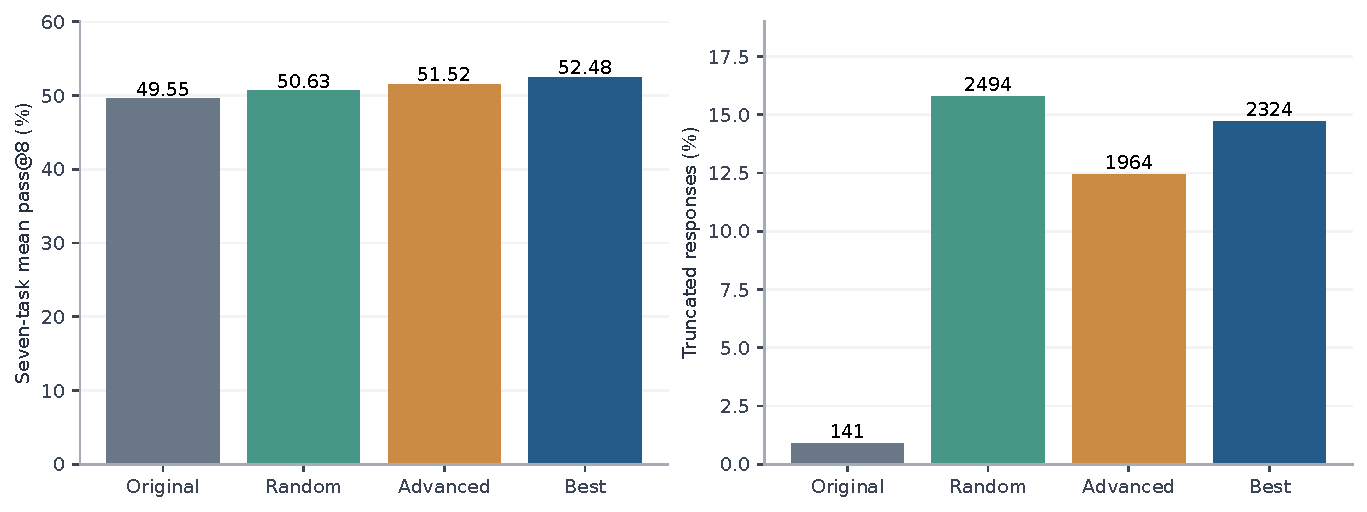
\includegraphics[width=\linewidth]{figures/rubric_tradeoffs.pdf}
\caption{Higher multiple-sample accuracy accompanies more length-limited responses. Count labels on the right use the same 15,792-response denominator.}
\end{figure}

\textbf{Stopping and single-sample reliability.} All trained models have lower seven-task pass@1 than the original, while their pass@8 rises. The best model has 2,324 truncated samples versus 141 for the original. Multi-attempt solving therefore improves numerically without establishing more reliable individual answers or better computational efficiency. Truncation alone does not show whether continued generations would become correct.

\textbf{Exploration and uncertainty.} Results come from a broader exploratory campaign and one training seed per reported model. No new confidence interval or statistical-significance claim is inferred from aggregate differences. Earlier advanced-versus-original paired bootstrap intervals remain in the repository, but they do not apply to the best-versus-random comparison. Sampling more questions cannot substitute for repeated training seeds or a preregistered confirmation.

\textbf{Selection proxies and confounds.} Lexical diversity does not validate reasoning, complete-looking answers can be wrong, and prefix-assisted success can reflect revealed answer information. The best model's larger context and three epochs confound a selection-only interpretation. Identifiable benchmark overlap is excluded, but semantic contamination and pretraining exposure remain possible. GPU constraints affected scheduling and follow-up scope; incomplete or timed-out evaluations are excluded from this table.

\textbf{Next experiments.} Compare selectors under equal context, token exposure, optimizer updates and initialization; repeat training seeds; and investigate response termination while preserving the evaluation prompt, sample count, token limits and grader. Ongoing work must finish independent audits and evaluation before replacing this snapshot. We do not forecast nine-benchmark success from training loss or partial results.

\newpage
\section{Reproducibility, Public Artifacts and Gaps}
\subsection{Repository and Artifact Identity}
The \href{https://github.com/rohitsalla/reasoning-sft-submission}{public GitHub repository} includes preparation/selection code, the vendored LLaMA-Factory trainer, portable training configurations, evaluator, shared protocol, score vectors, finite training histories, report source and figure builder. \texttt{REPRODUCE.md} provides environment setup, data preparation, training, inference and report commands. Training uses Transformers 4.55.0 and evaluation uses 4.57.6 in separate environments. Observed dependencies are recorded; they are not complete platform lockfiles or a bitwise replay guarantee.

The \href{https://huggingface.co/datasets/rohitspider/reasoning-sft-submission-data-15k}{public dataset release} contains both original random and advanced route exports. The \href{https://huggingface.co/rohitspider/reasoning-sft-submission-full-15k}{public full-model release} corresponds to the advanced route result of 51.5222\%, not the best assistance result of 52.4773\%. The downloader uses the readable release tag \texttt{course-submission-20261020-authors}.

\begin{itemize}
\item Best-model weights and the distinct assistance-selected export are not yet published. The best-run configuration and portable selector are included, but exact replay requires those missing artifacts and validated scoring observations.
\item Random-model weights are not published; its complete training history and nine-benchmark evaluation are included.
\item No official LiveBenchmark rank, top-five bonus or course-portal submission is asserted.
\end{itemize}

\subsection{Independent Outcome Checks}
A zero-GPU compute export verified that the four original manifests share the same inference protocol, hardware, dataset identities and question order. It recomputed all scores and truncations before exporting correctness and finish reasons. No raw generated reasoning or restricted question text was copied into the updated public evidence.

The public standard-library command \texttt{python3 scripts/verify\_submission.py} checks 7,896 records, 63,168 Boolean correctness flags, all four score tables, seven-task means, length-limited sample counts, complete finite random/best histories and the exact three-target count. Public record IDs are positional aliases for the privately verified common order. These checks recompute recorded outcomes; they do not rerun model inference, regrade raw responses or prove exported model-weight identity.

\section{Conclusion}
The completed core comparison gives a small descriptive pass@8 advantage to advanced route selection over random sampling. A separately trained assistance-and-coverage model is the best measured result at 52.4773\% seven-task pass@8 and three of nine fixed targets, with six targets still unmet. Worse truncation and lower pass@1 relative to the original qualify that result. The repository separates completed evidence from ongoing exploration and identifies missing artifacts, allowing assessment against the project rubric without implying complete nine-target success or official leaderboard standing.

\begin{thebibliography}{9}\small
\bibitem{qwen} Qwen Team. \emph{Qwen2.5-3B-Instruct model card}. \url{https://huggingface.co/Qwen/Qwen2.5-3B-Instruct}.
\bibitem{acereason} Dataset maintainers. \emph{AceReason-1.1 100K}. \url{https://huggingface.co/datasets/redsgnaoh/acereason11_100k}.
\bibitem{llamafactory} Y. Zheng et al. \emph{LlamaFactory: Unified Efficient Fine-Tuning of 100+ Language Models}. arXiv:2403.13372, 2024.
\bibitem{assignment} REDS Lab. \emph{Project-Reasoning-SFT-LLM assignment and evaluator}. \url{https://github.com/reds-lab/Project-Reasoning-SFT-LLM}.
\end{thebibliography}
\end{document}
